\section{Hvordan virker en vindmølle?}
Regeringens målsætning om $100 \%$ vedvarende energi i Danmark inden 2050 skal primært fuldføres med vinden som energikilde. 

\begin{wrapfigure}{r}{8.5cm}
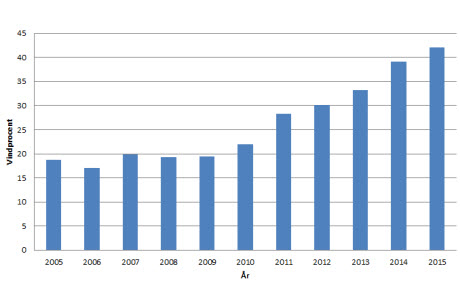
\includegraphics[width=8.5cm]{Billeder/vindgraf}
\caption{Figuren viser en graf over vindenergiens andel af den samlede energiproduktion \citep{2}}
\label{fig:vindgraf}
\end{wrapfigure}

Det ser også lyst ud, da energiproduktionen fra vindenergi i Danmark er vokset støt siden 2009. Her producerede de danske vindmøller $19,4 \%$ af den samlede danske energi produktion. Hvorimod at de i 2015 stod for hele $42,1 \%$ af den samlede produktion, hvilket kan ses på figur \ref{fig:vindgraf}. I 2016 led produktionen et lille fald til $37 \%$, hvilket var forårsaget af en væsentlig mindre mængde blæst end årene forinden. Fremover vil der dog komme flere vindmølleparker, hvilket får vindenergiens andel i den samlede produktion til at stige. \\
Udnyttelsen af vindenergi i Danmark sker primært med vindmøller af typen horisontal akslede hurtigløbere.
En hurtigløber er opbygget af flere forskellige komponenter, hvor de vigtigste heriblandt er rotoren, gearkassen, generatoren, lav- og højhastighedsakslen. Det er disse 5, der er med til at omdanne vindens kinetiske energi til en elektrisk effekt, som kan udnyttes af den danske elforbruger. \\
Processen starter med at vindmøllens vinger opfanger vinden. Når vinden passerer vingerne, kommer der en trykforskel omkring vingen, som giver en opdrift, hvilket får vingerne til at rotere. En grundigere forklaring af hvorfor vingerne begynder at rotere findes i teori afsnittet under Bernoullis ligning. \\
Når vingerne begynder at rotere, har vinden afgivet noget af sin kinetiske energi til vingerne, hvormed den er blevet omdannet til rotationsenergi. Vingerne er med rotoren forbundet til en lavhastighedsaksel, som med rotationsenergien fra vingerne får en gearkasse til at rotere. Gearkassen er forbundet videre til en højhastighedsaksel, som på grund af gearkassen roterer omtrent 50 gange så hurtigt som lavhastighedsakslen. Højhastighedsakslen driver vindmøllens generator, hvor induktion omdanner rotationsenergien til en elektrisk effekt. Vindmøllens samlede opbygning og hvordan de forskellige komponenter er forbundet kan ses på figur \ref{fig:vindmollen}.

\begin{figure}[H]
\centering
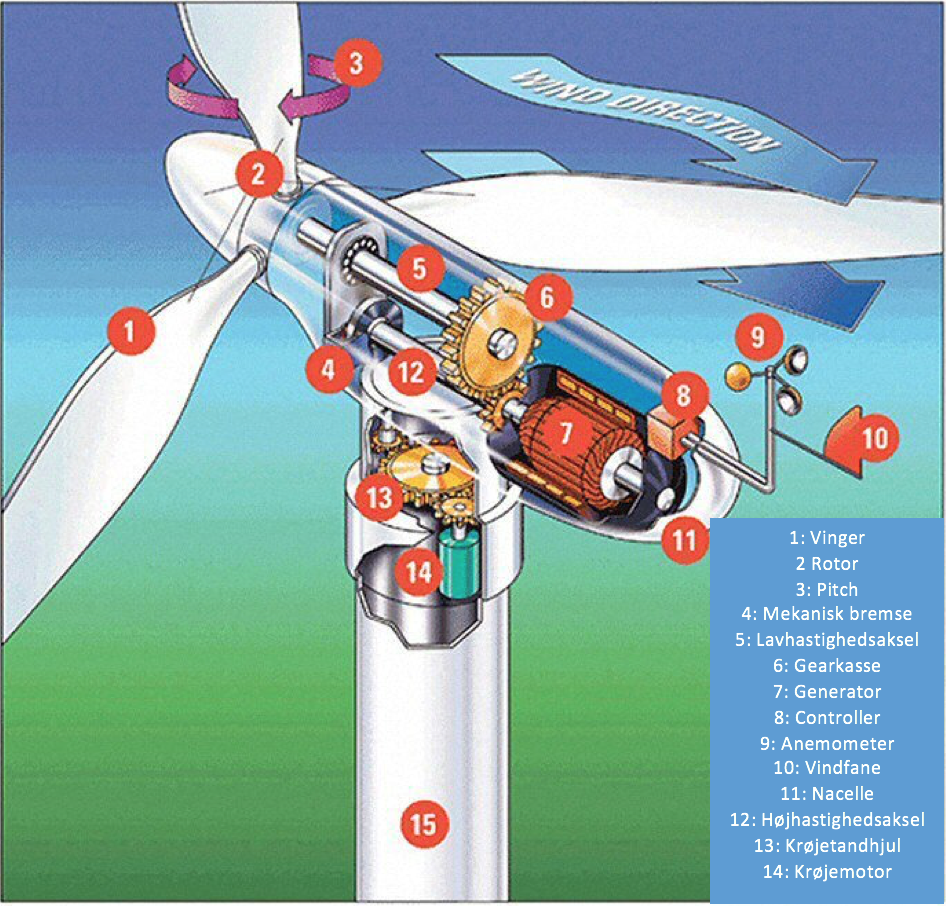
\includegraphics[width=0.80\textwidth]{Billeder/vindmollen}
\caption{Figuren viser komponenterne i en hurtigløber \citep{windturbine}.}
\label{fig:vindmollen}
\end{figure}

På figur \ref{fig:vindmollen} ses også vindmøllens krøjemotor. Det er denne motor, som drejer vindmøllehuset, så dens vinger står vinkelret mod vinden. Det er nemlig i denne position, at vindmøllen er mest effektiv. Hvornår og hvor meget vindhuset skal drejes for at indstille sig efter vinden afgøres af vindmøllens controller. Denne aflæser vindmøllens vindfane, begge kan ses på figur \ref{fig:vindmollen}. Selve rotorbladene kan også rotere en smule for at være i stand til  at slippe lidt ud af den i tilfælde af overproduktion. Funktionen kan også anvendes til at fange vinden bedre og gøre møllen mere effektiv, ligesom med krøjemotoren. 
Men selvom at man kan udnytte disse redskaber til at optimere energiproduktionen, ligger vindmøllens effektivitet mellem $35-45 \%$.
Effektiviteten bliver dog endnu lavere, når man tager højde for tab i blandt andet gearboksen og generatoren. Tages der højde for disse tab ender vindmøllen kun med at omdanne $10-30 \%$ af vindens kinetiske energi til en elektrisk effekt.
%http://www.raeng.org.uk/publications/other/23-wind-turbine
Dette er et godt stykke under det teoretiske maksimum udtrykt af Albert Betz i 1919. Han beviste, at det maksimalt er muligt at omdanne $59 \%$ af vindens kinetiske energi med vindmølletyper som en hurtigløber. En dybere gennemgang af dette kan findes i delen af teori afsnittet omhandlende Betz lov. 

Havde vindmøllen haft en effektivitet på $100 \%$, ville den tage alt energi ud af vinden, hvilket ville forårsage, at vindmolekylerne bremser fuldstændig op bag rotoren og blokerer passagen for de næste vindmolekyler. Dette medfører, at vindmøllen ville stoppe med at producere en effekt. 

Landskabet, hvor vindmøller placeres, har også en indflydelse på den producerede effekt. Omkring jordoverfladen er der flere forskellige faktorer, der kan spille ind og formindske udbyttet fra vindmøllen. Faktorer, der kan have en negativ indflydelse, kan for eksempel være skove, bjerge eller bygninger. Disse ting er både med til at give læ for vinden og samtidig skabe turbulens. Turbulensen sker typisk bag lægivere og er med til at få vindhastigheden til at variere både i hastighed og retning, hvilket medfører en nedsat produktion. 
Opstilles vindmøllen derimod på en græsmark eller det åbne hav vil vinden næsten ikke blive påvirket af landskabet. Begge overflader er forholdsvist glatte og vil tilnærmelsesvis ikke yde nogen modstand på vinden. 
De forskellige typer landskab kan inddeles i ruhedsklasser, som er med til at præcisere, hvor det er mest profitabelt at placere møllen. Ruhedsklasserne spænder mellem $0$ og $4$, hvor $0$ svarer til en vandoverflade og $4$ til en stor by med skyskrabere. 
Udover ruhedsklasserne har afstanden fra jordoverfladen og op til vingerne også en betydning for den producerede effekt. Jo længere væk vingerne befinder sig fra jordoverfladen, jo mindre bliver vinden påvirket af det omkringliggende landskab. Sammenhængen mellem højden og vindhastigheden kaldes for vindgradienten og kan afbildes med højden som funktion af vindhastigheden, hvor højden vil vokse eksponentielt, som en parabel. 
Det er altså både profitabelt at placere vindmøllerne steder med en ruhedsklasse så tæt på $0$ som muligt og/eller så højt som muligt. Dette er også grunden til, at der bliver oprettet så mange vindmølleparker ude på havet. Her er den eneste lægiver vindmøllerne selv og det er derfor ikke nødvendigt at bygge vindmøllerne alt for høje. 
Effekten havvindmøllerne producerer, ryger ud på elnettet og i sidste ende transporteret hen til forbrugeren. Effekten har altså en længere rejse undervejs i forhold til hvis nu, den blev produceret lokalt. Det gør den på de decentrale kraftværker, men i takt med at forbrændingen af fossile brændsler bliver udfaset, vil det være oplagt at opstille vindmøller eller anden form for vedvarende energi tæt på forbrugerne. I byerne er ruhedsklassen dog for høj og udover det er der også forskellige politiske regler, der umuliggører en eventuel opsætning af en vindmølle. 
Derfor vil det være fordelagtigt at opstille en invelox, da den med sit design vil blive mindre påvirket af de omkringliggende lægivere. Derudover er der endnu ikke opstillet nogle politiske begrænsninger angående dens størrelse og placering. 